\chapter{Secure (signed) Electronic Documents}

Let's start, as always with some definitions.
\begin{boxH}
  An \textbf{electronic document} is any \textbf{electronic
  representation} of a \textbf{document}, while a \textbf{digital
  document} is a \textbf{digital representation} of a document.
\end{boxH}

Secure electronic documents must satisfy the following properties:
\begin{itemize}
    \item \textbf{Security:} Ensure data integrity and authenticity
      using a digital signature.
    \item \textbf{Readability:} Use an open format for content and
      signature interpretation. This is crucial for long-term 
      archival: for example, we are having issue reading the data of
      the first Apollo mission.
    \item \textbf{Long-term Archival:} Ensure readability and
      verifiability over decades.
\end{itemize}

\section{Formats of Signed Documents}
Signed documents can take different formats:
\begin{itemize}
    \item \textbf{Enveloped Signature:} The signature is embedded
      within the document in a specific location (e.g., PDF).
    \item \textbf{Enveloping Signature(another case):} The document is
      embedded within the signature structure (e.g., PKCS\#7).
    \item \textbf{Detached Signature:} The signature is separate from
      the document (e.g., PKCS\#7). In this case the correlation
      between the signature of the document(for instance, using a
      pointer).
\end{itemize}

\begin{figure}[H]
  \centering
  \includegraphics[width=0.5\textwidth]{img/signed documents
  format.png}
  \caption{Different formats of signed documents.}
\end{figure}

\section{Multiple signatures}
In most case, multiple signatures are needed, for example in an office
there is typically a specific document workflow: an purchase order 
may need to be validated and approved by different people, each of 
which will sign the document in sequence(see figure \ref{fig:parrallel
signatures}). 

In those scenarios, the signatures can be either parallel or
sequential. In case of independent signature, each signature is applied
to the original document, meaning that the order of the signature is
irrelevant since each signature is indipendend from one another, while
in case of sequential signature, each signature is applied to the
previous signed document.
\begin{figure}[H]
  \centering
  \begin{subfigure}[b]{0.45\textwidth}
    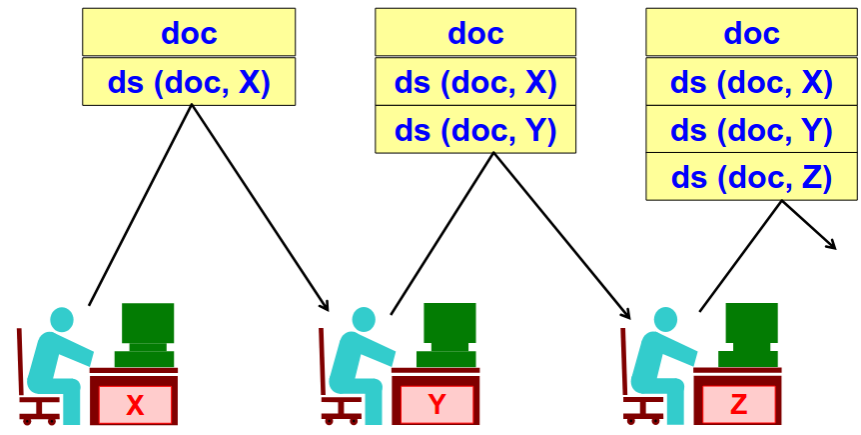
\includegraphics[width=\textwidth]{img/paralledl signatures.png}
    \label{fig:parrallel signatures}
    \caption{Parallel signatures in a single document.}
  \end{subfigure}
  \hfill
  \begin{subfigure}[b]{0.45\textwidth}
    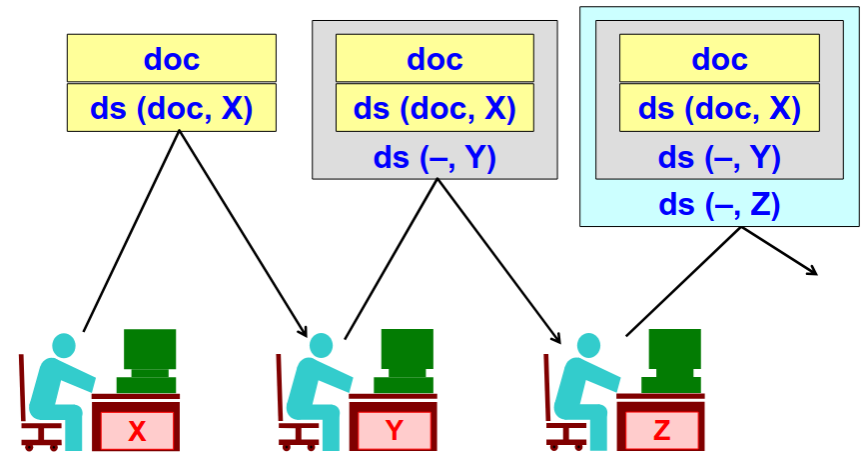
\includegraphics[width=\textwidth]{img/sequential signatures.png}
    \label{fig:sequential signatures}
    \caption{Sequential signatures in a single document.}
  \end{subfigure}
\end{figure}

\section{Digital Signatures in PDF Files}

When a PDF needs to be signed, it is at first converted in a byte
stream, while also reserving a specific place for the signature.
This allows to embed any kind of file format (even a movie) in a pdf 
file.

The data to be signed is identified by two intervals:
\begin{verbatim}
/ByteRange[ offset1, length1, offset2, length2 ]
\end{verbatim}
This divides the document in two parts, both of which are for the data
to allow the document to seem \textit{contiguous}.

Then, a digest of the data(signature excluded) is compute, for example
using sha-256, which is afterward encrypted with the signed private
key, via RSA-2048 for instance.

The signature value is encoded as a PKCS\#7 detached signature, and
the hex encoded signature value is inserted in the reserved space,
along with the necessary padding(made up of zeroes). This means that
even if technically the signature is detached from the document, in 
reality it is enveloped in the document.

If there's any leftover space in the reserved space, it is filled with 
zeroes.

\begin{figure}[H]
  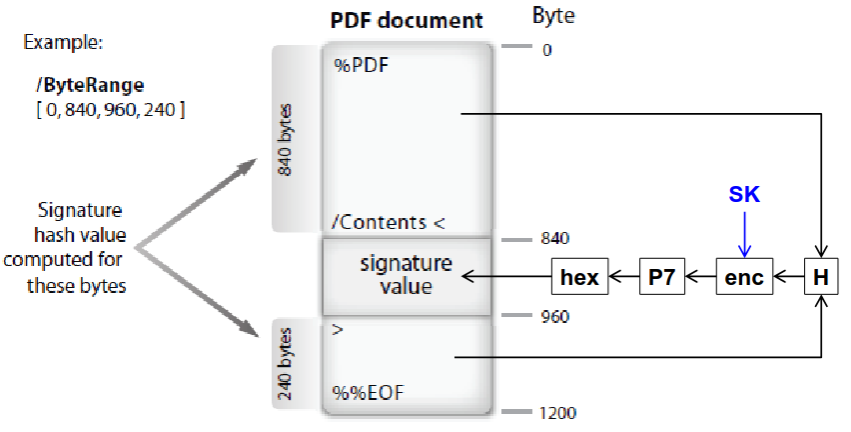
\includegraphics[width=.6\textwidth]{img/pdf digital signature.png}
  \caption{Digital signature in a pdf file}
  \label{fig:pdf digital signature}
\end{figure}


\section{Adobe Acrobat Signature Formats}
Adobe Acrobat supports the following signature formats:
\begin{itemize}
    \item \texttt{adbe.pkcs7.detached} (default).
    \item \texttt{adbe.pkcs7.sha1}.
    \item \texttt{adbe.x509.rsa.sha1}.
    \item \texttt{ETSI.CAdES.detached} (since Acrobat 10.x).
\end{itemize}
but also supports custom signature handlers, while retaining the same
structural format.

\subsection{Adobe Acrobat signature algorithms}
Adobe Acrobat provides support for various signature algorithms, which
evolve based on the Acrobat and PDF version. The details of supported
message digest algorithms and encryption or signature methods are as
follows:

\begin{itemize}
    \item \textbf{4.x–5.x} / PDF 1.3: MD5, SHA1
    \item \textbf{6.x} / PDF 1.3: MD5, SHA1
    \item \textbf{7.x} / PDF 1.6: MD5, SHA1, SHA256
    \item \textbf{8.x–9.0} / PDF 1.7: MD5, SHA1, SHA256, SHA384,
      SHA512, RIPEMD160
    \item \textbf{9.1–9.x} / PDF 1.7: MD5, SHA1, SHA256, SHA384,
      SHA512, RIPEMD160
    \item \textbf{10.x and later} / PDF 1.7: MD5, SHA1, SHA256,
      SHA384, SHA512, RIPEMD160
\end{itemize}

\subsection*{Encryption or Signature Algorithms}
\begin{itemize}
    \item \textbf{4.x–5.x} / PDF 1.3: RSA up to 1024-bit
    \item \textbf{6.x} / PDF 1.5: RSA up to 4096-bit
    \item \textbf{7.x} / PDF 1.6: RSA and DSA up to 4096-bit
    \item \textbf{8.x–10.x} / PDF 1.7: RSA and DSA up to 4096-bit
    \item \textbf{11.x and later} / PDF 1.7:
    \begin{itemize}
        \item RSA and DSA up to 4096-bit
        \item ECDSA P256-SHA256, P384-SHA384, or P512-SHA512
          (available only with \texttt{adbe.pkcs7.detached} and
          \texttt{ETSI.CAdES.detached})
    \end{itemize}
\end{itemize}

DSA supports only SHA1 (by design) and can only be used in
\texttt{adbe.pkcs7.detached}.

\subsection{Adobe Acrobat multiple signatures}
Since embedding another signature in the same document would require
overwriting the existing signature, Adobe Acrobat supports multiple
signature by associating them with incremental updates. This is
intewresting because a PDF usually keeps a history of the changes made 
to the document.

\begin{wrapfigure}{r}{0.4\textwidth}
  \centering
  \includegraphics[width=0.4\textwidth]{img/adobe multiple
  signatures.png}

  % \caption{CT System Configuration}
\end{wrapfigure}

\section{Electronic Signature (ES) and Advanced Electronic Signature
(AES)}
Electronic signatures are so important nowadays that the EU has
decided to standardize their format(not how they are created).
An ES is defined as:
\begin{boxH}
    Data in electronic form, attached to or logically associated with
    other electronic data, serving as a method of authentication.
\end{boxH}
This definition is quite broad to allow for different implementations 
and technologies.

On the other hand, an AES satisfies additional requirements:
\begin{itemize}
    \item Uniquely linked to the signatory, typically achieved by a
      asymmetric key pair.
    \item Capable of identifying the signatory, by using a public key
      certificate.
    \item Created under the signatory's sole control, by using a
      device in possession of the signatory, like a smart card.
    \item Detects any subsequent changes to the signed data, achieved
      by hashing the data.
\end{itemize}

\section{Qualified Certificate (QC)}
A Qualified Certificate (QC) is a PKC that certifies the identity of a
person. It includes specific attributes and information to ensure its
applicability for intended purposes. The main components of a QC are:

\begin{itemize}
    \item An explicit indication that it was issued as a Qualified
      Certificate.
    \item The name of the signatory or a pseudonym, clearly identified
      as such.
    \item Provision for specific attributes of the signatory, relevant
      to the certificate's intended purpose.
    \item Any limitations on the scope of the certificate, if
      applicable.
    \item Limits on the value of transactions, if applicable.
\end{itemize}

The QC is defined and profiled in \texttt{RFC-3739} under the
IETF-PKIX framework.

\subsection{Qualified Electronic Signature (QES)}
A QES is:
\begin{itemize}
    \item An AES based on a Qualified Certificate (QC).
    \item Created by a secure signature creation device.
    \item Legally equivalent to a handwritten signature.
\end{itemize}

Furthermore, notice that a QES is surely an AES, but the opposite is 
not necessarily true.

\begin{figure}[H]
  \centering
  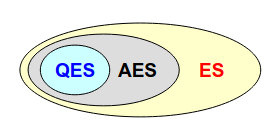
\includegraphics[width=0.4\textwidth]{img/es-aes-qus.png}
  \caption{Electronic Signature (ES), Advanced Electronic Signature
  (AES), and Qualified Electronic Signature (QES).}
\end{figure}

\section{Legal effects}
Member States shall ensure that an electronic signature is not denied
legal effectiveness and admissibility as evidence in legal proceedings
solely on the grounds that it is:
\begin{itemize}
  \item in electronic form, or
  \item not based upon a qualified certificate, or
  \item not based upon a qualified certificate issued by an accredited
    certification-service-provider, or
  \item not created by a secure signature-creation device
\end{itemize}

\section{ETSI Standards for electronic signature}
The European Union created the definitions for what is legally valid,
and then entrusted the ETSI to create the technical standards for the
implementation of those definitions.

ETSI standards for electronic signatures include:
\begin{itemize}
    \item \textbf{CAdES:} CMS Advanced Electronic Signatures.
    \item \textbf{XAdES:} XML Advanced Electronic Signatures.
    \item \textbf{PAdES:} PDF Advanced Electronic Signatures.
    \item \textbf{ASiC:} Associated Signature Containers for detached signatures.
\end{itemize}

\section{CAdES Formats}
\begin{itemize}
    \item \textbf{ES-C:} Includes complete certificate and revocation references.
    \item \textbf{ES-T:} Adds a timestamp over the digital signature.
    \item \textbf{ES-X:} Extends ES-C with additional timestamps for enhanced validation.
\end{itemize}


\section{Trust Service Status List (TSL)}
TSL is a signed list containing Trust-Service Providers (TSPs) and their services. It tracks the state (e.g., supervised, suspended) and history of each TSP.

\section{The "macro" problem}
As previously explained, the content of the PDF to be signed is
converted in a bytestream, and then signed. So if the bytecode is some
javascript, the code itself will be signed, and not the result of the
execution. This means that the signature will be valid even if the 
code is malicious. An this is a problem, because in some case the
macro will be evaluated and the macro code will be removed.

For exaple the Politecnico thesis archive requires a PDF/A format,
which is vulnerable to this kind of attack.

\section{WYSIWYS}
\textbf{What You See Is What You Sign (WYSIWYS)} ensures that the
displayed document content is what is actually signed. 
Think about very small clauses, or even the ones written with the same
color of the background. In this situations, this is an highly
desirable property, and it's not intrinsic to the digital signature 
itself.

Since this is not technically achievable by a digital signature alone,
from a legal standpoint, the signature may be considered invalid.

\section{The magic of Poste Italiane}
In the end, we use software to create a digital signatures, which is
usually buggy as a result of the complexity of the task. 

For example, in 2003, Postecom, which is the branch of Poste Italiane
that is managing certificates and the signature tool, which at the
time was \textit{Firma\&Cifra 1.0}, had a bug which accepted a root
certificate that was inside the PKCS\#7 document, with no check about
the root CA trustworthiness. This behaviour allowed for the creation
of a valid certificate for \textit{Arsene Lupin}, by even using a fake
root certificate for Poste Italiane, but at the time that
didn't have a CRL available so the signature was valid but the
verification was not.
\end{document}
